\documentclass[border=10pt]{standalone} 
\usepackage{tikz}

\usetikzlibrary{calc}
\usetikzlibrary{arrows}
\usetikzlibrary{shadows}
\usetikzlibrary{patterns}
\usetikzlibrary{positioning}
\usetikzlibrary{shapes}
\usetikzlibrary{3d}
%\usetikzlibrary{automata}
\usetikzlibrary{fit}

\tikzset{block/.style={draw, text centered, fill=gray!10,drop shadow}}
\tikzset{connect/.style={draw, line width=1 pt}}

\begin{document}

\beginpgfgraphicnamed{schema_mpu}

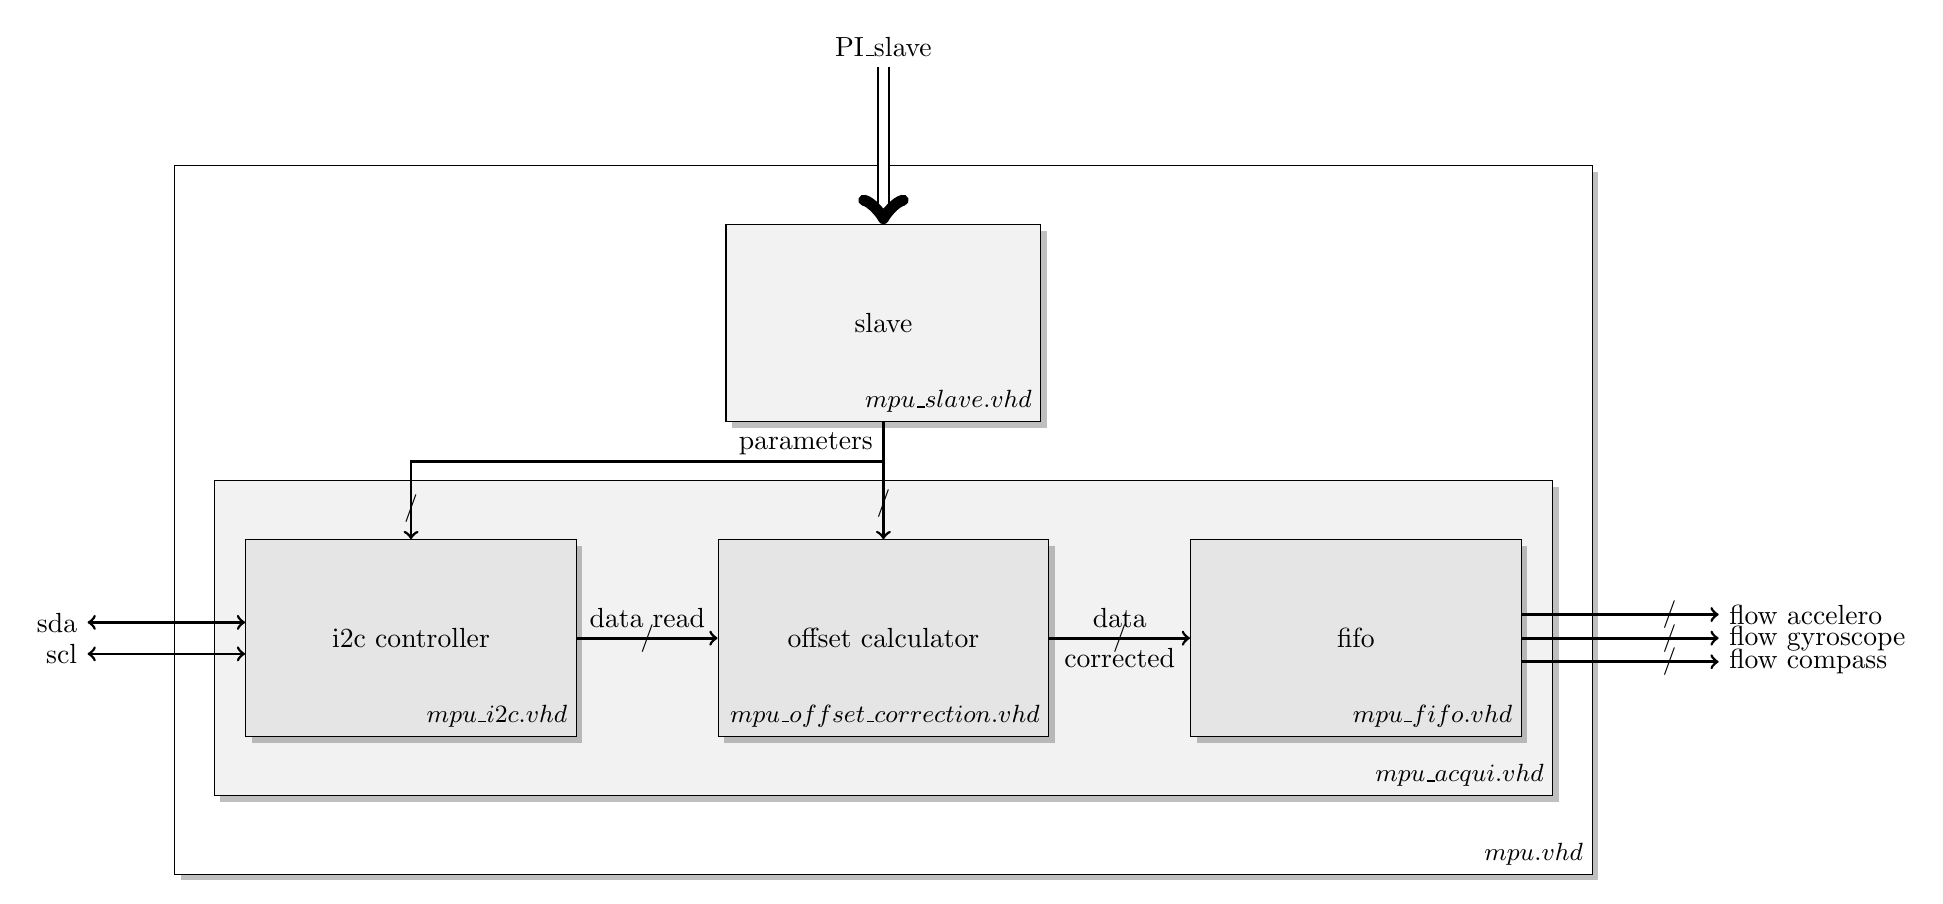
\begin{tikzpicture}



\node[block,minimum height=9cm,minimum width=18cm, fill=white] (bloc) {top\_MPU};
\draw (bloc.south east) node[above left]{\small $mpu.vhd$} ;

%sub block
\node[block,rectangle,minimum height=4cm,minimum width=17cm, fill=gray!10] (mpu) at([yshift=-1.5cm]bloc) {MPU};
\draw (mpu.south east) node[above left]{\small $mpu\_acqui.vhd$} ;

\node[block,rectangle,minimum height=2.5cm,minimum width=4.2cm,fill=gray!20] (i2c) at([xshift=-6cm]mpu) {i2c controller};
\draw (i2c.south east) node[above left]{\small $mpu\_i2c.vhd$} ;
\node[block,rectangle,minimum height=2.5cm,minimum width=4.2cm,fill=gray!20] (fifo) at([xshift=6cm]mpu) {fifo};
\draw (fifo.south east) node[above left]{\small $mpu\_fifo.vhd$} ;
\node[block,rectangle,minimum height=2.5cm,minimum width=4.2cm,fill=gray!20] (offset) at(mpu) {offset calculator};
\draw (offset.south east) node[above left]{\small $mpu\_offset\_correction.vhd$} ;

%external ports
\path[connect,<->] ([yshift=0.2cm]i2c.west) -- ++ (-2cm,0) node[left]{sda};
\path[connect,<->] ([yshift=-0.2cm]i2c.west) -- ++ (-2cm,0) node[left]{scl};

%signals in MPU
\path[connect,->] (i2c.east) --  node{/} node[above]{data read} (offset.west);
\path[connect,->] (offset.east) --  node{/} node[above]{data} node [below]{corrected} (fifo.west);

%flows out
\path[connect,->] ([yshift=0.3cm]fifo.east) -- node[near end]{/} ++(2.5cm,0) node[right]{flow accelero};
\path[connect,->] (fifo.east) -- node[near end]{/} ++(2.5cm,0) node[right]{flow gyroscope};
\path[connect,->] ([yshift=-0.3cm]fifo.east) -- node[near end]{/} ++(2.5cm,0) node[right]{flow compass};

%Slave and connections
\node[block,rectangle,minimum height=2.5cm,minimum width=4cm,fill=gray!10] (slave) at([yshift=2.5cm]bloc) {slave};
\draw (slave.south east) node[above left]{\small $mpu\_slave.vhd$} ;

\path[connect,<-][double distance = 3pt] (slave.north)  -- ++(0,2cm) node[above]{PI\_slave};


%parameters
\path[connect,->] (slave.south) node[below left]{parameters}  --  node[pos=0.7]{/} (offset.north);
\path[connect,->] ([yshift=-0.5cm]slave.south)  -| node[pos=0.8]{/}  (i2c.north);


\end{tikzpicture}


\endpgfgraphicnamed

\end{document}